
\chapter{Introduction}

\vspace{3mm}
% \noindent\rule{17cm}{0.2pt}
\fbox {
    \parbox{\linewidth}{
      \begin{itemize}
        \item Motivation and Aims
        \item Thesis outline
        \item Contributions to knowledge
      \end{itemize}
    }
}
\vspace{3mm}


\section{Motivation}


% cancer is bad
In the article titled "Is the world making progress against cancer?" \citep{Roser2015-qb}, the authors provide an overview of humanity's progress in combating the disease. Despite significant technological and biological advancements over the past decades, and an approximately 17\% reduction in standardised cancer death rates from 1990 to 2017, cancer remains a major global health challenge. As the world’s population continues to live longer, more people are being diagnosed with cancer, as reflected in the overall increase in cancer deaths (see \cref{fig}). Ageing is associated with the malfunction of normal physiological processes, which increases the likelihood of developing cancer. This underscores the ongoing prevalence of cancer and highlights the need for continuous development of new treatments to address the growing number of patients.


% Bladder cancer
According to Cancer Research UK \citeyearpar{Cancer_Research_UK2015-cf}, bladder cancer is the 10\textsuperscript{th} leading cause of cancer death, accounting for 3\% of all cancer-related deaths in the UK, with 56\% of cases occurring in people older than 75. Almost half (52.6\%) of those diagnosed with bladder cancer survive for more than five years, and 46.4\% survive for more than ten years. The treatments for bladder cancer require periodic medical check-ups as there is an increased recurrence rate, and in some instances, the bladder is removed. All of these aspects have a negative impact on the patient's quality of life and represent a burden for the healthcare system.

There are two major types of bladder cancer: \gls{NMIBC} (NMIBC) and \gls{MIBC} (MIBC). 9 out of 10 patients with NMIBC survive five years from the diagnosis, but there is a high chance of recurrence, which impacts the quality of life. MIBC is more aggressive than the other, with a higher chance of becoming metastatic and a worse 5-year survival rate of approximately 50\%. Bladder cancer is the 4\textsuperscript{th} most mutated cancer and suffers many epigenetic machinery modifications. The disruptions at multiple molecular levels make bladder cancer a challenging disease to study, and this project focuses on researching the subgroups of \acrlong{MIBC}.



\begin{figure}[!t]
    \centering
    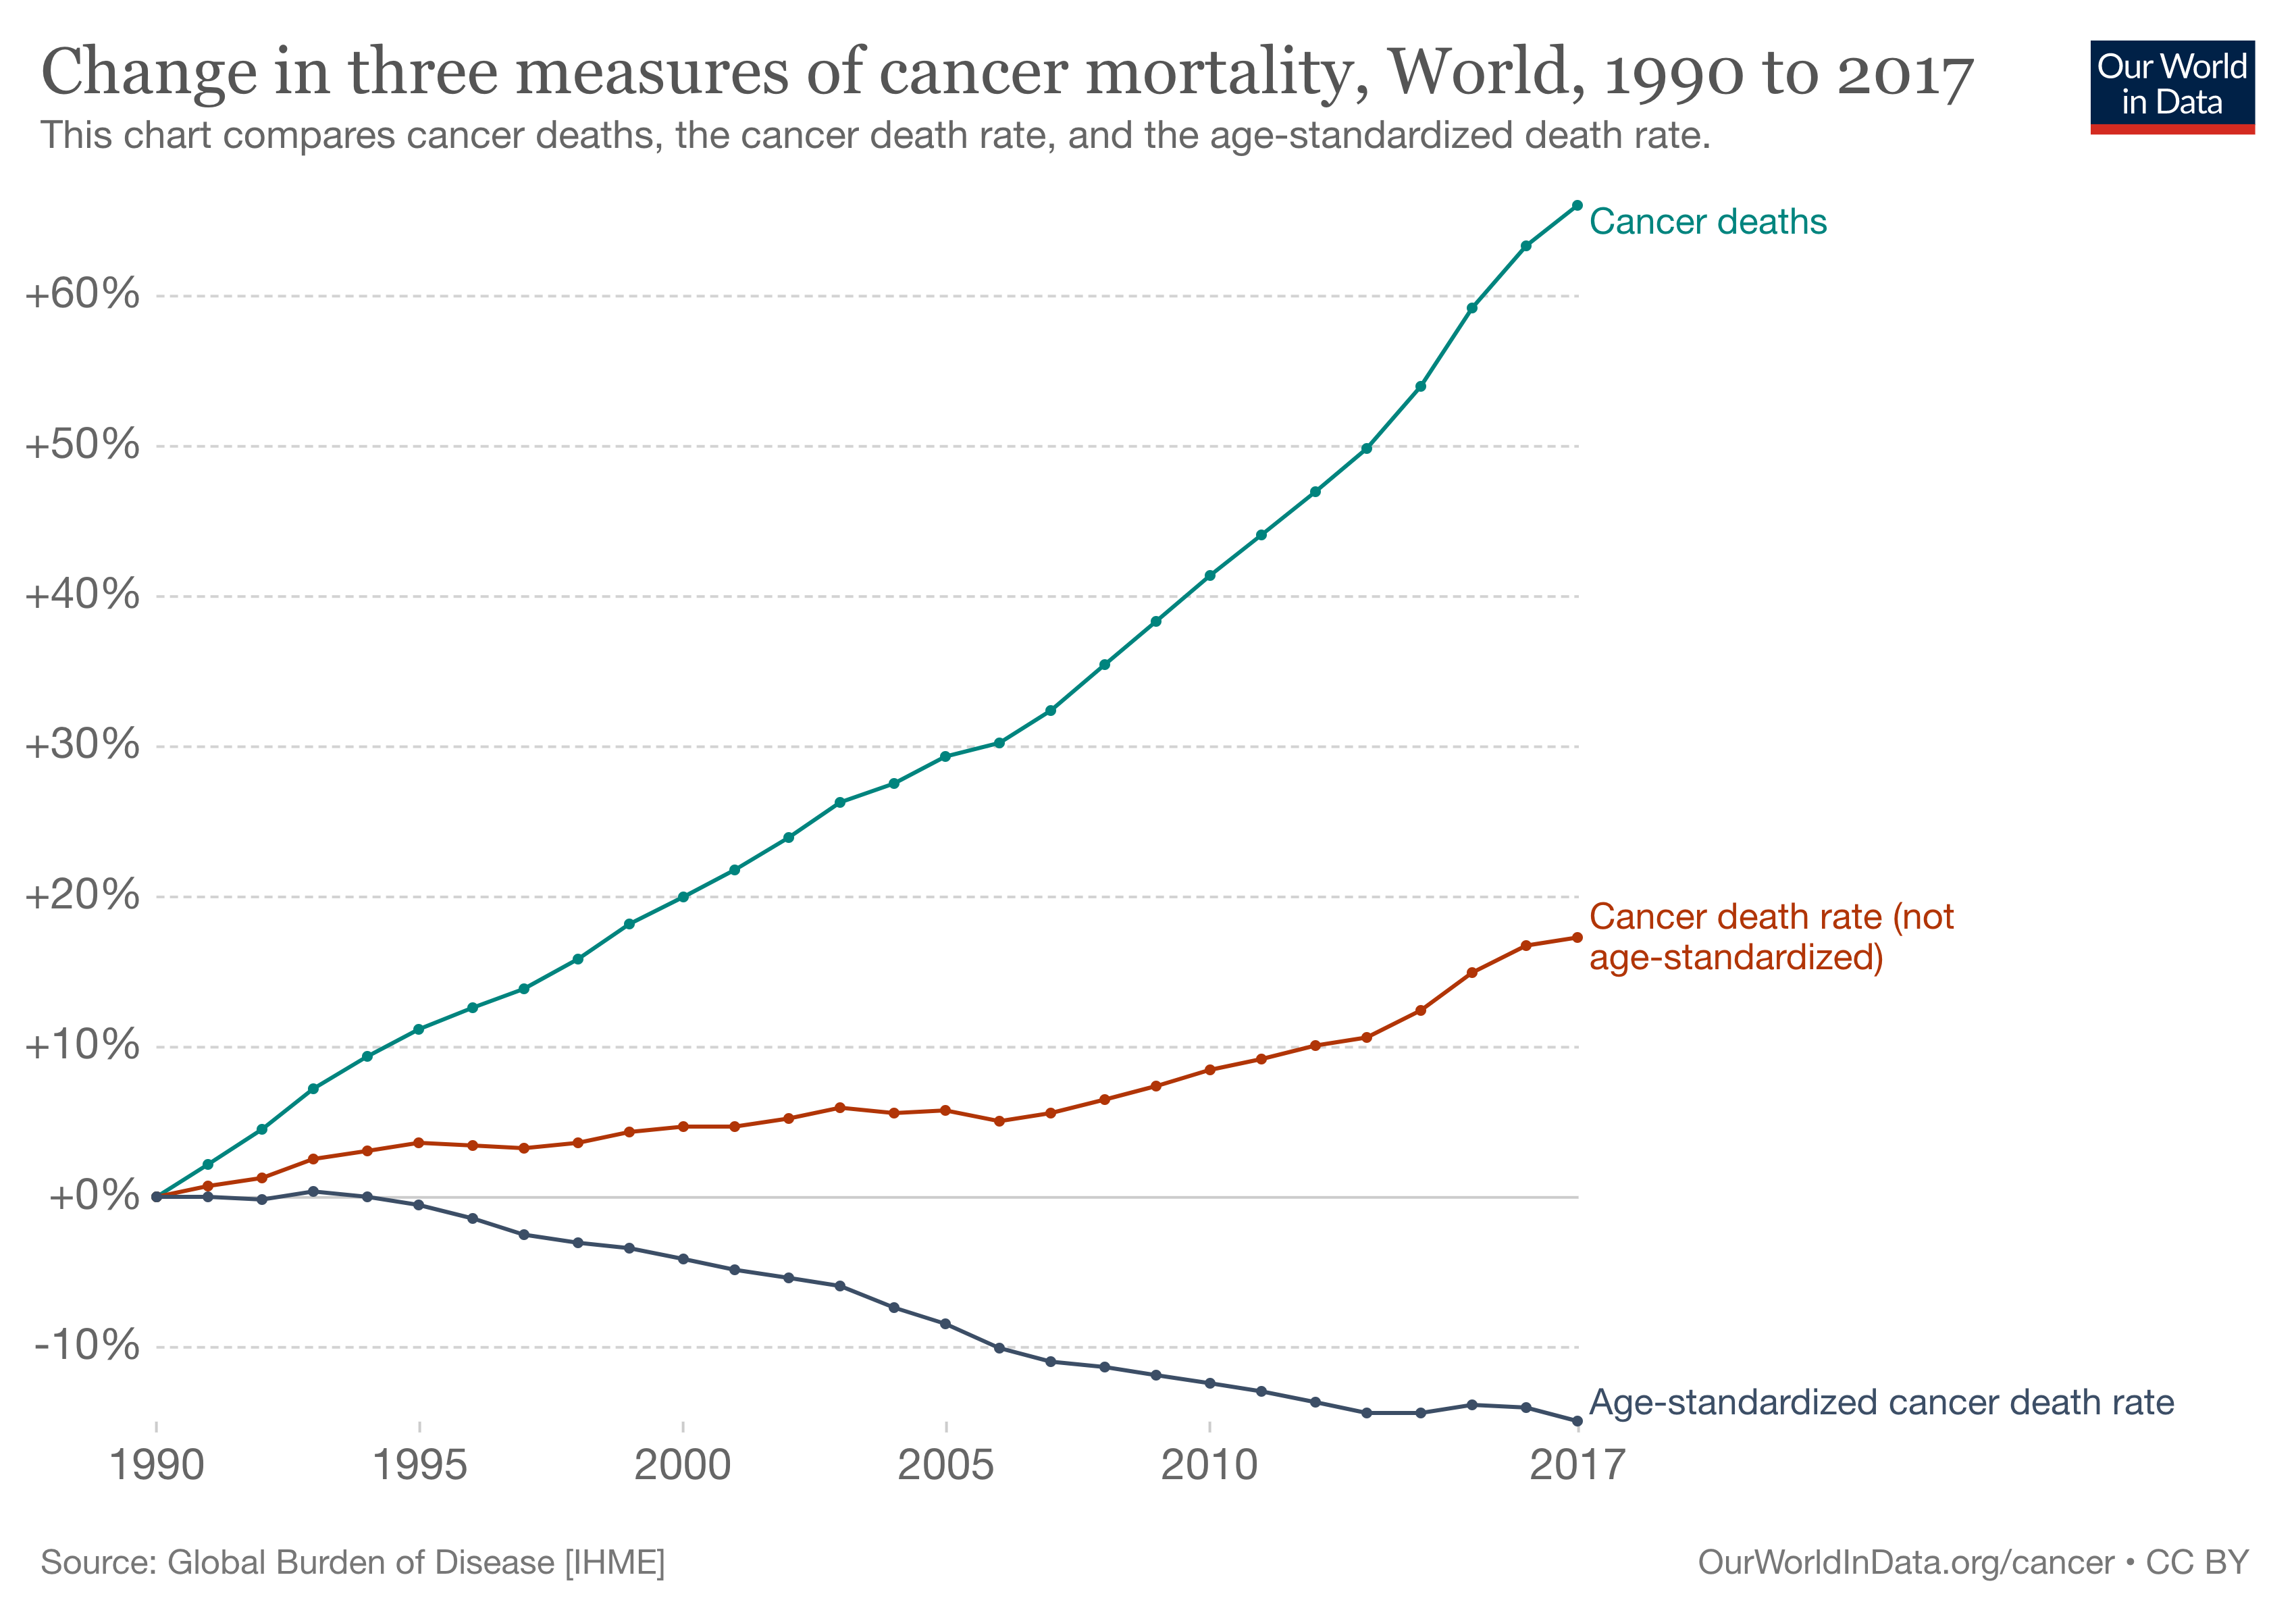
\includegraphics[width=0.8\textwidth,keepaspectratio]{Images/cancer-deaths-rate-and-age-standardized-rate-index.png}
    \caption[Cancer mortality]{With a more than 60\% increase in global cancer deaths over the past 30 years, cancer remains a major health challenge, despite advances in technology and medicine \citep{Roser2015-qb}.}
    \label{fig:cancer_death}
\end{figure}

% Limitations with MIBC classifications
\gls{GE}, or the abundance of the genes in the tumour tissue, is the primary data source for stratifying MIBC \citep{Kamoun2020-tj,Robertson2017-mg,Marzouka2018-ge}. The aim of finding subgroups of the disease is to improve treatments by developing more targeted solutions, a step towards personalised treatments. However, while there are some clinical trials \citep{Griffin2024-zr} underway, these subgroups have yet to significantly improve clinical outcomes. One reason is that other tumour information, such as anomalies (mutations) or epigenetic modifications, is analysed separately and then attributed to the groups identified through gene expression.

% What we're doing
Therefore, the motivation of this project is to address the limitations of current \gls{MIBC} stratification by developing a new integrative network approach to stratify \gls{MIBC} in a way that is translatable to the clinic.


% While some clinical trials \citep{Griffin2024-zr} are underway, these subgroups have yet to improve clinical outcomes significantly. The complex molecular characteristics of MIBC necessitate the development of subtypes based on multi-omics data integration.


\section{Aims} \label{s:intro:aims}


% The project's hypothesis proposes that integrating additional data types into the gene expression data will result in MIBC subtypes that more accurately represent the molecular biology of the samples. Especially by combining the gene expression of the non-tumour samples with the mutations and expressed genes in the tumour, it will lead to new MIBC subgroups. Based on this, the project aims can be defined as follows:

The current MIBC subtypes are based only on tumour expression data without considering the other available data types \citep{Kamoun2020-tj, Robertson2017-mg}. However, this is a complex type of cancer where normal processes malfunction at different levels. Thus, it is hypothesised that using gene expression from non-tumour (healthy) samples into which integrated mutation and regulatory information will lead to new and different MIBC subgroups with a closer representation of biology. These subgroups will then help advance bladder cancer research and develop targeted treatments. Based on this hypothesis, the project aims can be defined as follows:

\begin{enumerate}
    \item Create a method that allows the integration of multiple data types
    \item Utilise non-cancerous gene expression to inform tumour classifications
    \item Enable researchers to trace the biological mechanisms behind each subtype
\end{enumerate}

While working on achieving the research aims stated above, the research was guided by the following principles:

\begin{itemize}
    \item Traceability - allows the researchers to understand and explain the outputs of the approach used
    \item Ensure the method is modular and tissue-agnostic, allowing its application to other diseases
    \item Keep the software and the method complexity to a minimum, the complexity arises from the biology
    % \item Keep the software and method as simple as possible, ensuring that any complexity is driven by the underlying biological data
    \item Develop a platform that enables the integration of additional data types beyond those considered in this PhD project
\end{itemize}

% Thesis outline
\section{Thesis Outline}

\textbf{Background (\cref{s:lit_review_intro})} - This chapter introduces the reader to the current state of research on MIBC and the various classification systems found in the literature. It continues by presenting the datasets and methods used in the project, followed by a review of disease stratification methods beyond bladder cancer and gene expression. The final two sections of the chapter cover network methods used in biological applications and community detection methods for identifying subgroups within a network.


\textbf{Cluster Analysis (\cref{s:clustering_analysis})} - This thesis section delves deeper into the clustering methods used throughout the project, whether to group gene expression data or network outputs. Through a standard clustering analysis process, we discovered that one of the major MIBC groups, the basal subtype, can be further divided into three subgroups with differing immune responses and survival prognoses. Notably, the subgroup with the lowest immune response has the poorest 5-year survival rate.

\textbf{A Network Pipeline for Subtyping (\cref{s:N_I})} - This research investigates the integration of data into a network approach at three key stages: 1) modelling edge weights proportional to the genes' mutation burden in MIBC, 2) selective edge pruning, which allows Transcription Factors (TF) to have more connections than other genes, and 3) using gene expression from freshly isolated samples to build a co-expressed network. 
The chapter assesses the impact of these data integration strategies on the network's metrics.


\textbf{Selective Edge Pruning (\cref{s:N_I:sel_pruning})} - This chapter extends the previous work in the project, focusing on finding the appropriate configuration for the number of edges assigned to Transcription Factors genes and comparing the Leiden community detection algorithm with \acrfull{sbm}. From the selective edge pruning experiments, 98 TF were identified as naturally co-expressed with other genes, even in a control network. Using the tumour gene expression of this subset to stratify the TCGA's MIBC cohort, a Basal subgroup formed of 7\% of samples from the tumour cohort was discovered, characterised by the lowest survival prognosis in the literature. Notably, this subgroup does not contain samples previously classified as \acrlong{ne} and exhibits squamous phenotypes. \acrshort{sbm} is preferred for community detection as it identifies more communities and is robust in detecting patterns in random data.


\textbf{Network II (\cref{s:N_II})} - It introduces a refined network approach where the data integration methods from Chapter 4 are improved to have a larger impact on the network. Compared to the work from \cref{s:N_I}, the network is built from a larger number of healthy samples and the mutation burden of the MIBC is gradually integrated into edge weight modifiers. The research presented identifies 122 genes (TF and non-TF) concentrated in small communities (\(<\)10 nodes) that are highly and strongly correlated, as well as having a high mutation burden. The analysis showed that many of the significantly differentially expressed genes are \acrlong{lncRNA} genes, which do not encode for proteins, making them understudied in cancer subtyping but recent studies show that these have a regulatory role \citep{Statello2021-md}. This indicates the added level of complexity and information by using the healthy gene expression representation and the limits of current biological knowledge.


\textbf{Discussion \& Future Work (\cref{s:discussion})} - This chapter presents the significance and implications of the findings throughout the project and discusses potential avenues for future research.


% Contribution to knowledge
\section{Contributions of each chapter}

Below is a succinct summary of the findings in each of the results chapter that is meant to guide the reader and improve the reading experience.

\paragraph*{Cluster analysis (\Cref{s:clustering_analysis})}

The work in this chapter was presented at the International Bladder Cancer Network (IBCN) conference from Barcelona in 2022.


\begin{itemize}
    \item Three basal subgroups with heterogeneous \acrfull{ifn} immune response
    \item The basal group with the lowest immune response exhibits the worst 5-year survival rate
    \item The basal samples with a strong \acrshort{ifn} response show a more favourable prognosis and can represent potential treatment targets
    \item An aggressive gene filtering of the expressed genes contributes to the findings of the new Basal 
\end{itemize}

\paragraph*{Network I (\Cref{s:N_I})}

\begin{itemize}
    \item Validates the network approach as an integrative method for MIBC stratification
     \item Integration of the mutation burden and TF affect the network, community detection and MIBC stratification
     \item Network generated from the gene expression obtained from freshly isolated cells finds different groups from the tumour network representation
\end{itemize}

\paragraph*{Selective Edge pruning (\Cref{s:N_I:sel_pruning})}

The research covered in this chapter was presented at the Complex Networks (CN) conference from Menton, France in 2023.

\begin{itemize}
    \item Selective edge pruning as a method to find highly correlated genes in gene expression datasets 
    \item 98 TF drive a three-way basal split
    \item The Basal group of 20 samples exhibiting squamous markers has the lowest survival prognosis seen in the project and possibly in the literature
    \item Compares two classes of community detection methods in the biological networks
\end{itemize}

\paragraph*{Network II (\Cref{s:N_II})}

This chapter brings the following contributions to the field:
\begin{itemize}
    \item A more advanced network pipeline is used to form a healthy (non-tumour) network representation from which the \acrshort{mibc} is informed
    \item Identification of a subset of genes and communities with a high mutation burden, which are highly and strongly co-expressed with other genes
    \item \acrfull{hsbm} from the network pipeline finds small communities off less than 10 genes in a network of 5000 nodes
    \item Discovery of new \gls{BASAL} and \gls{LUMINAL} subdivisions: the former has a low survival rate, and the latter has the highest survival rate over five years. Both are characterised by communities with Ensembl genes,
    \item Identifying new splits in the ABS-Ca and P0 datasets which are enriched by some of the same communities with Ensembl genes from previous point 
    \item An explainable computational solution which allows tracing the result (i.e. subtyping) to network communities and implicitly to a subset of genes
    \item Across the analysis, many differentially expressed genes were found to be Ensembl genes, highlighting the potential for discovering new biological insights
    \item Development of a Python package that gene the network, which is planned to be released to the research community
\end{itemize}